%%
%% Beginning of file 'sample.tex'
%%
%% Modified 2005 December 5
%%
%% This is a sample manuscript marked up using the
%% AASTeX v5.x LaTeX 2e macros.

%% The first piece of markup in an AASTeX v5.x document
%% is the \documentclass command. LaTeX will ignore
%% any data that comes before this command.

%% The command below calls the preprint style
%% which will produce a one-column, single-spaced document.
%% Examples of commands for other substyles follow. Use
%% whichever is most appropriate for your purposes.
%%
%%\documentclass[12pt,preprint]{aastex}

%% manuscript produces a one-column, double-spaced document:

%\documentclass{article}
%\documentclass[twocolumn]{aastex6}
\documentclass{aastex6}
%\documentclass[iop]{emulateapj}

%% preprint2 produces a double-column, single-spaced document:
%\documentclass[preprint2]{aastex}

%% Sometimes a paper's abstract is too long to fit on the
%% title page in preprint2 mode. When that is the case,
%% use the longabstract style option.

%% \documentclass[preprint2,longabstract]{aastex}

%% If you want to create your own macros, you can do so
%% using \newcommand. Your macros should appear before
%% the \begin{document} command.
%%
%% If you are submitting to a journal that translates manuscripts
%% into SGML, you need to follow certain guidelines when preparing
%% your macros. See the AASTeX v5.x Author Guide
%% for information.

%Packages
%\usepackage[colorlinks=true,linkcolor=blue,citecolor=blue]{hyperref}
\usepackage{graphicx}
\usepackage{float}
%\usepackage{caption}
%\usepackage{subcaption}
\usepackage[caption=false]{subfig}

\usepackage{natbib}
%\usepackage{pdflscape}
\bibliographystyle{astroads}

\newcommand{\vdag}{(v)^\dagger}
\newcommand{\DHSres}{299 - 334}
\newcommand{\DHSresApprox}{300}
\newcommand{\DHSgap}{0.04}
\newcommand{\degree}{^\circ}
\newcommand{\SOSSrange}{0.6 - 2.5~$\mu$m}
\newcommand{\SOSSrangeto}{0.6 to 2.5~$\mu$m}

%% You can insert a short comment on the title page using the command below.

\slugcomment{\textcolor{red}{NOTE, this is will be morphed into a paper appendix}}

%% If you wish, you may supply running head information, although
%% this information may be modified by the editorial offices.
%% The left head contains a list of authors,
%% usually a maximum of three (otherwise use et al.).  The right
%% head is a modified title of up to roughly 44 characters.
%% Running heads will not print in the manuscript style.

\shorttitle{Distant Suns}
\shortauthors{Schlawin et al.}

%% This is the end of the preamble.  Indicate the beginning of the
%% paper itself with \begin{document}.

\begin{document}

%% LaTeX will automatically break titles if they run longer than
%% one line. However, you may use \\ to force a line break if
%% you desire.

\title{Distant Suns for JWST Flux Calibration}

%% Use \author, \affil, and the \and command to format
%% author and affiliation information.
%% Note that \email has replaced the old \authoremail command
%% from AASTeX v4.0. You can use \email to mark an email address
%% anywhere in the paper, not just in the front matter.
%% As in the title, use \\ to force line breaks.

\author{E. Schlawin, G. Rieke, Christopher Willmer, Jarron Leisenring, M. Rieke, K. Misselt}
\affil{Steward Observatory, Tucson AZ 85721}
\email{eas342@email.arizona.edu}

%% Notice that each of these authors has alternate affiliations, which
%% are identified by the \altaffilmark after each name.  Specify alternate
%% affiliation information with \altaffiltext, with one command per each
%% affiliation.

%\altaffiltext{1}{Hubble Postdoctoral Fellow}

%% Mark off your abstract in the ``abstract'' environment. In the manuscript
%% style, abstract will output a Received/Accepted line after the
%% title and affiliation information. No date will appear since the author
%% does not have this information. The dates will be filled in by the
%% editorial office after submission.

\begin{abstract}
The James Webb Space Telescope (JWST) offers unprecedented sensitivity and stability for science.
Most science areas in astronomy require flux calibration in order to convert brightness measurements into physical flux units.
We discuss a program to identify solar analog calibrators at the low end of the flux scale that will not saturate most wide-band NIRCam imaging in full frame mode and that can also be used with other Science Instruments for faint calibration.
We identified two star clusters: NGC~2420 and NGC~2506 to be the best balance of extinction, age, distance and metallicity, where solar type stars can be used for calibration.
We use NGC~2506 for Cycle 1 JWST flux calibration due to its faintness, which saturates the fewest number of modes.
We include a catalog of sources and absolutely calibrated photometry in the $K$ band using the WFCAM instrument on UKIRT.
%$g$, $r$, $i$, $z$, $J$, $H$, $K$ and IRAC1 3.6 $\mu$m bands.
We provide a small catalog of solar type stars within 1 spectral type of G2V from ground-based optical spectroscopy.
These faint calibrators serve wide band full frame imaging of JWST as well as future ground-based imagers.
\end{abstract}

%% Keywords should appear after the \end{abstract} command. The uncommented
%% example has been keyed in ApJ style. See the instructions to authors
%% for the journal to which you are submitting your paper to determine
%% what keyword punctuation is appropriate.

\keywords{instrumentation: spectrographs}

%% From the front matter, we move on to the body of the paper.
%% In the first two sections, notice the use of the natbib \citep
%% and \citet commands to identify citations.  The citations are
%% tied to the reference list via symbolic KEYs. The KEY corresponds
%% to the KEY in the \bibitem in the reference list below. We have
%% chosen the first three characters of the first author's name plus
%% the last two numeral of the year of publication as our KEY for
%% each reference.


%% Authors who wish to have the most important objects in their paper
%% linked in the electronic edition to a data center may do so by tagging
%% their objects with \objectname{} or \object{}.  Each macro takes the
%% object name as its required argument. The optional, square-bracket 
%% argument should be used in cases where the data center identification
%% differs from what is to be printed in the paper.  The text appearing 
%% in curly braces is what will appear in print in the published paper. 
%% If the object name is recognized by the data centers, it will be linked
%% in the electronic edition to the object data available at the data centers  
%%
%% Note that for sources with brackets in their names, e.g. [WEG2004] 14h-090,
%% the brackets must be escaped with backslashes when used in the first
%% square-bracket argument, for instance, \object[\[WEG2004\] 14h-090]{90}).
%%  Otherwise, LaTeX will issue an error. 

\section{Introduction}

The James Webb Space Telescope \citep[JWST; e.g.][]{gardner2006SSRv} will need absolute calibration to accomplish its science goals with a calibration program outlined in \citet{gordon2022absFlux1}.
One area where accurate flux calibration is especially important is dark energy science, which makes use of type Ia supernovae as standard candles.
Absolute fluxes are especially important for improving type Ia supernova luminosity distances and thus the expansion history of the Universe \citep[e.g.][]{narayan2016wdnetwork,betoule2014cosmologySN}.
For exoplanet host stars in the era of Gaia distances, absolutely calibrated photometry is used to make precision measurements of stellar radii, which in turn give high precision planet radii \citep[e.g.][]{stassun2017gaiaRadiiMasses}.
JWST will have no standard calibration sources onboard so all calibration must be performed with astronomical sources.

The JWST flux calibration effort has been described in \citet{gordon2009fluxplan1}, \citet{gordon2011fluxplan2} and \citet{gordon2022absFlux1}.
Figure \ref{fig:JWSTcalsWideF} shows several of the sources that are planned as targets for flux calibration.
These include three categories: 1) hot stars (white dwarf and OB stars) 2) G-stars (which are solar-like) and 3) A-type stars.
The variety of spectra used in JWST calibration can mitigate against biases when models are used to convert flux in one filter to the expected flux in another filter.

The original flux calibration effort has mainly bright stars ($K \lesssim 15$).
Example spectra for these calibrators are shown in Figure \ref{fig:JWSTcalsWideF} with saturation and sensitivity limits of NIRCam's wide filters.
Many of these spectra will saturate the NIRCam detectors when used in full frame (shown as the middle parts of the black ``error bars'') for wide-band filters.
Furthermore, there may be systematic errors when observing faint targets and low detector well depths.
As an example of a systematic detector effect, consider charge traps within a detector.
These traps would tend to decrease the measured number of electrons per second on the first exposure because they would trap electrons  that would not be read out by an amplifier.
For bright sources, the effect of the traps would be smaller since they would quickly be a small fraction of the flux.
For faint sources, however, the traps would be a larger fraction of the incoming electrons.
Therefore, the charge traps (if not corrected for) would tend to decrease the flux of faint sources as compared to bright targets.

\begin{figure}[!hbtp]
\centering
%\includegraphics[width=.48\columnwidth]{nircam_wide_filters.png}
\includegraphics[width=.48\columnwidth]{calspec_and_new_clust.pdf}
\includegraphics[width=.48\columnwidth]{calspec_and_new_clust_niriss.pdf}
\caption{CALSPEC models are plotted in comparison to JWST saturation and sensitivity limits for NIRCam (left) and NIRISS (right), as shown in \citet{gordon2011fluxplan2}.
The three values shown for each wideband filter are the subarray saturation (upper error limit), full frame saturation (middle circle) and 10~$\sigma$ sensitivity limit in one hour of imaging (lower error limit).
Three classes of JWST calibrators are shown: hot stars including white dwarfs (blue), A-type stars (green) and G-type stars (red).
Additional faint calibrators are needed to extend the sample from \citet{gordon2011fluxplan2} towards the faint limits of NIRCam.
We discuss an effort to add G2~V type stars in open clusters to the calibration sample.
Example G2~V \citet{castelli2004models} models are shown for stars expected in the three clusters NGC~6811, NGC~2420 and NGC~2506.
}\label{fig:JWSTcalsWideF}
\end{figure}

In this paper, we discuss a JWST Flux Calibration Working Group effort to identify and calibrate stars to add to the JWST sample on the fainter end at $K \approx 15.4$ to $K \approx 16.3$.
We use the solar analog method \citep{rieke2008absIRcal,johnson1965solarAnalogMethod,megessier1995solarAnalogCal} for flux calibration.
The basic rationale is that the Solar spectrum is well measured across JWST's wavelengths \citep[0.6~$\mu$m to 29~$\mu$m][]{gardner2006SSRv} and has highly accurate models for its spectrum \citep[e.g.][]{gueymard2018solarSpectrum}.
When solar-like stars are identified, one can use these models to convert from one photometric or spectroscopic band to another.
We identify solar-like stars in open clusters because it allows us to average over multiple stars and to cross-calibrate with bright references within the cluster.
The color magnitude diagram of the cluster also allows us to identify solar like stars and aids in the corrections for extinction.

\section{Cluster Properties}

Our team examined open clusters from the WEBDA database\footnote{https://www.univie.ac.at/webda/webda.html} to find clusters most suitable for flux calibration with solar-like stars.
The parameters under consideration were the the following:
\begin{itemize}
\item {\bf Age:} For the methods to work, the solar-mass stars must be on the main sequence. If we require that a solar mass star have $T_{\rm eff}$ = 5780 +/- 100 K, the cluster would have to be between 0.3 Gyr and 10 Gyr using Dartmouth evolutionary models \citep{dotter2008dartmouth}. Furthermore, the age should be $\lesssim$7 Gyr to avoid main sequence turnoff of F-type stars that have similar colors to solar analogs.
\item {\bf Extinction} Extinction should be as small as possible to minimize the effects of extinction correction to photometry. Of the clusters found, E(B-V) $\lesssim 0.1$.
\item {\bf Distance Modulus} The clusters should be distant enough that they do not saturate NIRCam or NIRISS wide-band imaging in full frame mode. The most easily saturated wide band filter for G stars is the F090W, which corresponds to a G2~V star of 15.9 in the $K$ band.
While the F150W2 ``double-wide'' filter is more easily saturated than F090W, this is filter is not used as widely in extragalactic surveys, where the wide filters are preferred for photometric redshift \citep[e.g.][]{williams2018JWSTMockCatalog}.
This means the true distance modulus $(m - M)_0$ should be 12.6 for a solar absolute K=3.27 \citep{willmer2018solarMagnitude}.
The longer wavelength wide band filters (F200W, F277W, F356W, and F444W) will not saturate for a true distance modulus larger than 11.8.
If one assumes an extinction of E(B-V) = 0.05 and a Galactic average extinction law \citep{cardelli1989}, the visual distance modulus $(m- M)_V$ should be an additional 0.15 mag.
Thus, to calibrate all wide band filters longer than F200W in full frame mode, the visual distance modulus $(m- M)_V$ should be larger than 11.95.
\item {\bf Metallicity} Ideally, the cluster should have near-solar metallicity so that the solar mass stars have a luminosity near 1 $L_\sun$ and a G2~V type spectrum.
\item {\bf Compactness} The cluster should be relatively compact compared to NIRCam's FOV (2'$\times$2' per module).
We selected clusters with WEBDA diameters $\lesssim 15\arcmin$
\item {\bf Ancillary data} The clusters should have ancillary photometry from multiple observatories for cross-calibration. We preferred clusters with 2MASS, WISE and IRAC measurements.
\item {\bf Visibility} The clusters should be spread out in ecliptic longitude to ensure that at least one is visible during the commissioning period.
\end{itemize}

No cluster could meet all criteria but some had a balance of desirable properties.
With all these considerations in play, we selected NGC 2420 and NGC 2506 as the best fit for the multiple criteria.
The only parameter that is not satisfied by NGC 2420 is the distance modulus, so additional sources or conversions are needed for the F070W, F090W, F115W and F150W filters.
At the time NGC 2420 was selected, the JWST throughputs were smaller than the measured values so it saturated fewer filters.
One way to calibrate these short wavelength, wide filters is to use subarrays.
The subarray to full frame conversion can be checked with medium band filters.
NGC 2420 has -0.05 $\le$ [Fe/H] $\le$ 0.04.
NGC 2506, is metal poor at [Fe/H]=-0.32, so corrections must be made for changes to G2 V spectra due to metallicity.

%\begin{figure}
%\centering
%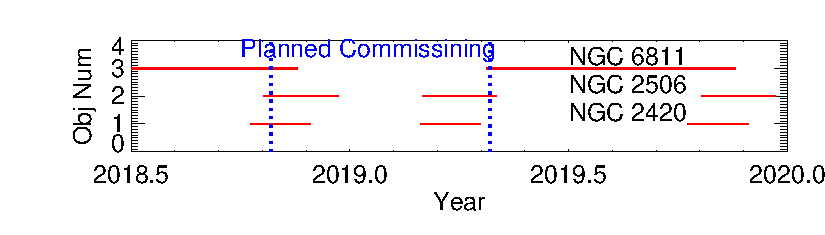
\includegraphics[width=.4\columnwidth]{cluster_visibilty.pdf}
%\caption{Visibility windows for the three open clusters considered in this report.
%The planned commissioning period is shown with vertical blue dashed lines.}\label{fig:clusterVis}
%\end{figure}

These clusters also allow for accurate calibration of MIRI imager with solar analogs.
For example, a typical G2~V star in NGC~2420 can be measured in the MIRI F1000W filter with a signal to ratio of about 150 in 1000 seconds of integration.
Although this integration time is considerably longer than for NIRCam imaging, they are still comparable to the 1800 second slew time charged in APT.
Thus, it should require a smaller time allocation for a 1000 sec MIRI flux standard observation than two flux standards separated in the sky with NIRCam.

After selecting the sources, we discovered that the WEBDA database had parameters that were significantly different from the literature for these individual clusters.
%For example E(B-V)$_\mathrm{WEBDA}$ = 0.16 for NGC 6811 whereas \citet{molendaz2016spec6811} has E(B-V) = 0.05.
We therefore did a literature search for the most recent available cluster parameters.
Table \ref{tab:clusterProp} shows the properties gathered from the literature.
Recent literature values indicate that both clusters have low extinction with E(B-V) $<$ 0.1.

\begin{table}
\centering
\caption{Cluster Parameters}\label{tab:clusterProp}
\begin{tabular}{lrrrrc}
\hline \hline
Cluster   					&  E(B-V) 			& Distance Mod 	& [Fe/H] 			& Age 		& Distance\\
          					&     				&    (m - M)$_V$	& 	dex 			& Gyr 		& kpc	\\
\hline \hline
NGC 2420\tablenotemark{b}	& 0.04 $\pm$0.03	&  11.88 $\pm$ 0.27	& -0.05 $\pm$ 0.03	& 3 $\pm$ 1 	& 2.2 $\pm$ 0.3 \\
NGC 2506\tablenotemark{c}	& 0.080 $\pm$ 0.006	&  12.71\tablenotemark{a}	 	& -0.36 $\pm$ 0.10			& 2.01 $\pm$ 0.10 & 3.101 $\pm$ 0.017 \\
%NGC 6811\tablenotemark{d}	& 0.05 $\pm$0.02	& 10.29 $\pm$ 0.14	& 0.04 $\pm$ 0.01 	& 1.0 $\pm$ 0.1 & 1.1 $\pm$ 0.1 \\
\hline
\end{tabular}
%\caption{G2V-type star saturation K band limits are shown for suggested sub-array sizes. The size affects the number of DHS that can be included, so the noise in the DHS spectra over 1.1 -- 1.9$\mu$m at the given saturation limit for a 1 hour transit is shown in column 4 at native R $\sim$ \DHSresApprox\ resolution.}\label{tab:SatSNRsubA}
\tablenotetext{a}{Distance calculated by taking the visual distance modulus $(m-M)_V$ and subtracting the expected extinction for a Galactic average extinction law  \citep{cardelli1989} applied to a 5800 K star.}
\tablenotetext{b}{NGC 2420 parameters from \citet{pancino2010chem2420}.}
\tablenotetext{c}{NGC 2506 parameters from \citet{knudstrup2020ngc2506properties}}
%\tablenotetext{d}{NGC 6811 parameters from \citet{molendaz2016spec6811}}
\end{table}

\section{Photometry}\label{sec:photometry}
\subsection{Pan-Starrs Photometry}\label{sec:panStarsPhot}

We obtained $grizy$ Pan-Starrs photometry \citep{magnier2013photLadder,schlafly2012photcal,tonry2012panstarrsPhot} for all both clusters.
We also estimated the Pan-Starrs $g$ - $r$ and B-V colors from a Pickles G2~V spectrum using \texttt{pysynphot} \citep{lim2015pysynphot}, the measured extinction shown in Table \ref{tab:clusterProp} with a Milky Way Diffuse R(V)=3.1 \citet{cardelli1989} extinction law.
Figure \ref{fig:cmdPS} shows the Pan-Starrs and \citet{janes2013keplerPhot} color magnitude diagram for the three clusters along with vertical bars with the expected solar color for each cluster: $g-r$ =0.42 and $g-r$ = 0.43 for NGC~2420 and NGC~2506 respectively.
We identified main sequence stars by fitting an iterative sigma clipped 5th polynomial to the color as a function of magnitude.
We then included all points within 0.04 mag and 0.03 mag from the polynomial as main sequence stars for NGC~2420 and NGC~2506, respectively.

We created 3 levels of priority in assigning slit fibers (MMT Hectospec, NGC~2420) or slit masks (Keck LRIS~NGC 2506).
The highest priority targets were the ones with $g-r > 0.3$ and $g-r \le0.45$ for NGC~2420 and $g-r > 0.38$ and $g-r \le 0.48$ for NGC~2506.
We also prioritized targets within  $2 \times 4\arcmin $ for NGC~2420 and $9.5 \times 9.5\arcmin $ for NGC~2506 (based on the LRIS field of view).
These priority levels preferred fiber or mask selection of stars within a small field of view most close to a G2V spectrum.

\begin{figure*}[!t]
\centering
\subfloat[NGC 2420]{
	\includegraphics[width=0.5\textwidth]{sources_ngc2420.png}
	\label{fig:cmdNGC2420}
	}
\subfloat[NGC 2506]{
	\includegraphics[width=0.5\textwidth]{sources_ngc2506.png}
	\label{fig:cmdNGC2506}
	}
\\
%\subfloat[NGC 6811]{
%	\includegraphics[width=0.5\textwidth]{sources_ngc6811.png}
%	\label{fig:cmdNGC6811}
%	}
	\caption{Color-magnitudes of the two clusters.
	The main sequence in each cluster was fit with a polynomial and then three priority levels were chosen for follow-up spectroscopy.
	The first priority targets were near-solar $g-r = 0.42-0.43$ or ($\pm 0.04, 0.03$ for NGC~2420 and NGC~2506, respectively) that were within $\pm$4\arcmin\ of the cluster center (to concentrate in the Science Instrument field of view).
	The second priority were near-solar $g-r$ or B-V colors but with a wider field of view (1$\degree$) to include G2~V stars that could be observed with larger dithers.
	Thirdly, any remaining main sequence stars that were within the 1$\degree$ hectospec field of view with reasonable signal to noise were selected to allow for errors in photometric color predictions and enable star cluster science at the main sequence turnoff point.}
	\label{fig:cmdPS}
\end{figure*} 

\subsection{UKIRT Photometry}

We observed both clusters with WFCAM on the UKIRT telescope in queue mode on October 11,25, 26, November 11 and December 29, 2016 (UTC).
This is the same instrument, pipeline and telescope for the UKIDSS survey for the infrared $JHK$ bands.
The data were processed automatically by the CASU IR Reduction Software (CIRDS) version 1.202 \citep{irwin2004vistaDataFlowWFCAM}, which created photometric catalogs for every detector array.
We focused primarily on the one detector centered on the cluster.
As recommended by the UKIRT pipeline team (Mike Irwin, private communication), we used aperture photometry number 3 (1\arcsec\ radius) for the fluxes in the J, H and K bands.

\subsection{Tie-in to 2MASS Photometry}

We identified over 1000 WFCAM sources in common with the 2MASS survey \citep{skrutskie06}.
We used these overlapping stars to check for offsets between the 2MASS survey on the WFCAM photometry, as shown in Figure \ref{fig:ukirtVs2MASS}.
Fainter than $K=14$ gets into the low signal to noise regime for 2MASS, whereas $K<11.5$ approaches saturation with WFCAM, so the stars between those ranges are the most useful on cross-checking photometry.
We find an offset of UKIRT K - 2MASS K = 0.007 if using all 2MASS and WFCAM points with $11.5 < K \le 14$.


\begin{figure}[!hbtp]
\centering
\includegraphics[width=.9\columnwidth]{ukirt_2mass_NGC_2506.pdf}
\caption{A comparison of UKIRT and 2MASS photometry for cross-matched sources.}\label{fig:ukirtVs2MASS}
\end{figure}
%
%Straight Horzontal Lines
%Median UKIRT J - 2MASS J = -0.0090
%from  1356 points
%Median UKIRT H - 2MASS H = 0.0130
%from  1320 points
%Median UKIRT K - 2MASS K = 0.0255
%from  1084 points

%Median of all crossmatched points with K $>$ 12 and $| UKIRT - 2MASS | < 0.2$.


\clearpage
\section{Spectral Typing of Candidate Analogs}

\subsection{Hectospec Observations}\label{sec:hectoObs}

We used the Hectospec instrument on the MMT \citep{fabricant2005hectospec,mink2007hectoFibers} to obtain spectra of candidate solar analogs in NGC~2420.
We observed NGC~2420 with two fiber configurations in the Spring and Fall of 2016.
We used the 600 gpm grating (1.9 - 2.2 $\AA$ resolution element) to match with existing spectral template libraries with 3.6 $\AA$ resolution.
We selected the central wavelength to be 4800 $\AA$ which means that the wavelength coverage is about 3550 to 6050 $\AA$, which covers several import features for G-star classification many of which are concentrated between 4000 and 4400 $\AA$.
We obtained exposure times of 1.7 hours (Spring 2016) and 2 hours (Fall 2016).
The minimum fiber separation $\sim$20$\arcsec$ required that we observe in two configurations to increase the density of stars for which we had spectral classification.
During the observing run in the Fall of 2016, the 600 gpm (1.9 - 2.2 $\AA$ resolution element) grating had to be removed for repairs and so we were forced to observe NGC 2506 with the 270 gpm (4.5 - 5.2 $\AA$ resolution element).
The spectral typing uncertainty grows with lower resolution.

We processed the data with the standard IDL routine \texttt{HSRED}\footnote{https://www.mmto.org/node/536}, which applies automatic bias and flat field corrections, spectral extraction and wavelength calibration.
\texttt{HSRED} can apply flux calibration for F-type stars, but we elected to rectify the spectra.
Flux calibration is not crucial to spectral typing G-type stars since the spectrum is relatively flat in the optical (Chris Corbally, priv. communication).

We normalized the raw spectra output from \texttt{HSRED} in order to pass it to a spectral rectification program \texttt{mkclass} \citep{gray2014classification}.
The first step in the normalization was to get an approximately normalized curve from the strongly curved spectrum shown in Figure \ref{fig:SpecRect}.
We fit a cubic spline in log space to the flux as a function of wavelength.
The fit is iterated 3 times with 2$\sigma$ outlier rejection to account for strong spectral lines and cosmic rays.
It is important to do the fit in log-space because in linear space there are regions (near 3800 $\AA$) where the best-fit polynomial drops to low values and the fit can have zero crossings.
If this cubic spline model (fit in linear space) is used to rectify the spectrum, the rectified spectrum will have large negative values or NaNs when divided by the model, whereas the fit in log-space has no zero-crossings.

The second step in the spectral rectification process is to normalize by the pseudo continuum and remove any residual curvature.
This is again fit with a cubic spline with 3 iterations of outlier rejection.
The modification for the second step is to do it in linear space (now that zero crossings will not occur) and also select only points greater than 0.95 to ensure they are continuum points.
The two steps (with cubic spline fits) and final resulting spectrum are shown for an example source in Figure \ref{fig:SpecRect}.

\begin{figure}[!hbtp]
\centering
\includegraphics[width=.7\columnwidth]{images/O_0738284_p2131_spec.pdf}
\caption{The Hectospec spectra are rectified in two steps 1) to take out the strong curvature with a robust cubic spline in log flux space (top panel) and 2) to fit the points above 0.95 with a cubic spline in linear flux space.
The resulting spectrum is used for classification.
In this example for the source at 07:38:28.5 +21:31:39.7, spectral classification with \texttt{mkclass} eventually gives a spectral type of F8 IV.}\label{fig:SpecRect}
\end{figure}

\subsection{Keck LRIS Observations}\label{sec:keckLRIS}
We observed NGC~2506 on December 6, 2018 with Keck LRIS using custom slit masks, with target priority outlined in Section \ref{sec:panStarsPhot}.
We designed masks with slit widths of 0.7\arcsec $\times$ 5\arcsec, which matched well to the seeing on December 6, 2018 near 0.7\arcsec.
We used the D560 dichroic and 600/4000 grating to collect blue spectra from 330 nm to 560 nm, which includes the temperature sensitive absorption lines from 400 to 450 nm.
The slit and grating combination resulted in a resolution of $\sim$0.3 nm for our slit widths or smaller in the case of good seeing.
The LRIS red arm was not used for spectral typing.
We took dome flats and HgNeArCdZnKrXe  arc lamp exposures for wavelength calibration and direct observations of NGC~2506 field for source identification and alignment.

We used the \texttt{pypeit} pipeline to extract spectra of all sources \citep{prochaska2020pypeit}.
Some additional adjustments were needed to find spectral types of the stars.
A -35 km/s velocity (wavelength) adjustment correction was needed to shift all spectra to match the stellar templates from the \texttt{mkclass} \citep{gray2014classification} library.
As with the Hectospec data described in Section \ref{sec:hectoObs}, we rectify the spectra by fitting to a third order spline with a 2$\sigma$ iterative clipping rejection and 4 splin knots.

Figure \ref{fig:SpecRectLRIS} shows the rectified spectra for one of the slit masks with several temperature-sensitive lines highlighted.

\begin{figure}[!hbtp]
\centering
\includegraphics[width=.7\columnwidth]{all_spec_good_wavecal_2019-02-06-07_combined_spec_maskAnR1_rectified.pdf}
\caption{Rectified LRIS spectra of Solar Analog candidates are shown for one slit mask.}\label{fig:SpecRectLRIS}
\end{figure}

\clearpage
\subsection{Spectral Classification}

We used the automatic ``expert'' classification system \texttt{mkclass} \citep{gray2014classification} to classify the stars.
This program is different from automated neural networks in that it directly uses the same methods as a human classifier does, rather than being trained on a specific set of data.
The \texttt{mkclass} programs comes with a library of standards at 3.6$\AA$ resolution standards and 1.8$\AA$ standards.
Our Hectospec data with the 600 gpm grating has a spectral resolution of 1.9 to 2.2$\AA$ so we convolve it with a Gaussian kernel to match the 3.6$\AA$ library.
Our Keck LRIS data have a spectral resolution near 0.3$\AA$, so we use the 0.22$\AA$ spectral template library.
We use 3 iterations, the \texttt{mkclass} default.

\begin{figure}[!hbtp]
\centering
\includegraphics[width=.49\columnwidth]{colormagNGC_2420.pdf}
\includegraphics[width=.49\columnwidth]{fovNGC_2420.pdf}
\caption{{\it Left:} A color magnitude diagram from the Pan Starrs photometry of NGC~2420 with the sources that were observed with Hectospec and classified by \texttt{mkclass}.
The G2~V sources line up with with the expected solar $g-r$ from a Pickles G2~V spectrum (red vertical line).
{\it Right} The field of view of the Pan-Starrs photometry over-plotted with the same sources.
Two rectangles are drawn to represent the field of view of the NIRCam module A and module B. Up to 3 G2~V sources may be observed simultaneously with NIRCam and more can be included with a dither pattern.
The NIRISS field of view is similar to one of NIRCam's modules and could observe 2 G2~V sources at a time. }\label{fig:ngc2420ClassCM}
\end{figure}

Figure \ref{fig:ngc2420ClassCM} shows the spectral types output by \texttt{mkclass} in both color-magnitude space as well as the field of view with boxes to represent the NIRCam arrays for NGC~2420.
A single pointing could include 3 G2~V sources and more can be covered with a dither pattern.
In \ref{fig:ngc2420ClassCM} we compare the observed Pan-Starrs colors of the G2~V spectral type stars to a Pickles library spectrum.
After applying a R(V)=3.1 \citet{cardelli1989} Milky Way Diffuse extinction law with E(B-V)=0.04, the Pickles spectrum lines up very closely (within 0.021) of the expected $g-r$=0.042.

We show the final color magnitudes for NGC~2420 and NGC~2506 in Figure \ref{fig:finalCandidatesCM} after selection of spectroscopically confirmed near-G2V $pm$ 1 temperature class for targets that are within a compact field of view.

\subsection{Visual Classification}

The \texttt{mkclass} classifications of near-solar stars were checked by eye, which is a helpful verification for \texttt{mkclass} (Chris Corbally, private communication).
A graphical user interface explorer was made to compare template classification spectra with the observed Hectospec spectra\footnote{https://github.com/eas342/mkclassfication\_viewer}.
Figure \ref{fig:0738284p2133class} shows the Hectospec spectrum of a source at 07:38:28.4 +21:33 that \texttt{mkclass} identifies as G2~V.
The line ratios of Ca I 4226~$\AA$, H$\delta$, H$\gamma$ and Fe I lines are most consistent with a G2 V type, within 1 temperature class.

\begin{figure}[!hbtp]
\centering
\includegraphics[width=.95\columnwidth]{O_0738284_p2133_class_g2v.pdf}
\caption{An example G2~V source found by \texttt{mkclass} (07:38:28.4 +21:33) is visually checked against spectral templates.
Of particular importance for temperature classification are the Ca I 4226~$\AA$, H$\delta$, H$\gamma$ and Fe I lines highlighted above \citep{gray2009specClass}.
Two standards (G2 V and G1.5 V) are shown for comparison.}\label{fig:0738284p2133class}
\end{figure}



\begin{figure*}[!t]
\centering
\subfloat[NGC 2420]{
	\includegraphics[width=0.5\textwidth]{colormag_NGC_2420_near_G2_V.pdf}
	\label{fig:cmdNGC2420nearG2V}
	}
\subfloat[NGC 2506]{
	\includegraphics[width=0.5\textwidth]{colormag_NGC_2506_near_G2_V_g-r.pdf}
	\label{fig:cmdNGC2506nearG2V}
	}
%\\
%\subfloat[NGC 6811]{
%	\includegraphics[width=0.5\textwidth]{colormag_NGC_6811_near_G2_V.pdf}
%	\label{fig:cmdNGC6811nearG2V}
%	}
%	\caption{Color-magnitudes of the three clusters with the near-solar stars identified from spectra.
%	}
%	\label{fig:cmdPSnearG2V}
\end{figure*}\label{fig:finalCandidatesCM}


\clearpage

\section*{Acknowledgements}
%\acknowledgments

Thanks to Dani Kiminki and John Stauffer for the selection of open clusters for this work and for finding targets based on initial data.
Thanks to Richard Gray and Chris Corbally for their help in stellar classification and guidance with the Hectospec observations.
Funding for the NIRCam team is provided by NASA Goddard Spaceflight Center. This research has made use of the WEBDA database, operated at the Department of Theoretical Physics and Astrophysics of the Masaryk University.
Observations reported here were obtained at the MMT Observatory, a joint facility of the University of Arizona and the Smithsonian Institution.
This paper uses data products produced by the OIR Telescope Data Center, supported by the Smithsonian Astrophysical Observatory.
The Pan-STARRS1 Surveys (PS1) have been made possible through contributions of the Institute for Astronomy, the University of Hawaii, the Pan-STARRS Project Office, the Max-Planck Society and its participating institutes, the Max Planck Institute for Astronomy, Heidelberg and the Max Planck Institute for Extraterrestrial Physics, Garching, The Johns Hopkins University, Durham University, the University of Edinburgh, Queen's University Belfast, the Harvard-Smithsonian Center for Astrophysics, the Las Cumbres Observatory Global Telescope Network Incorporated, the National Central University of Taiwan, the Space Telescope Science Institute, the National Aeronautics and Space Administration under Grant No. NNX08AR22G issued through the Planetary Science Division of the NASA Science Mission Directorate, the National Science Foundation under Grant No. AST-1238877, the University of Maryland, and Eotvos Lorand University (ELTE) and the Los Alamos National Laboratory. 

%If used, some data was collected from the Open Exoplanet Catalogue \citep{rein2012openExoCat}.

%% In a manner similar to \objectname authors can provide links to dataset
%% hosted at participating data centers via the \dataset{} command.  The
%% second curly bracket argument is printed in the text while the first
%% parentheses argument serves as the valid data set identifier.  Large
%% lists of data set are best provided in a table (see Table 3 for an example).
%% Valid data set identifiers should be obtained from the data center that
%% is currently hosting the data.
%%
%% Note that AASTeX interprets everything between the curly braces in the 
%% macro as regular text, so any special characters, e.g. "#" or "_," must be 
%% preceded by a backslash. Otherwise, you will get a LaTeX error when you 
%% compile your manuscript.  Special characters do not 
%% need to be escaped in the optional, square-bracket argument.



%% In this section, we use  the \subsection command to set off
%% a subsection.  \footnote is used to insert a footnote to the text.

%% Observe the use of the LaTeX \label
%% command after the \subsection to give a symbolic KEY to the
%% subsection for cross-referencing in a \ref command.
%% You can use LaTeX's \ref and \label commands to keep track of
%% cross-references to sections, equations, tables, and figures.
%% That way, if you change the order of any elements, LaTeX will
%% automatically renumber them.

%% This section also includes several of the displayed math environments
%% mentioned in the Author Guide.


%% The equation environment wil produce a numbered display equation.


%% The \notetoeditor{TEXT} command allows the author to communicate
%% information to the copy editor.  This information will appear as a
%% footnote on the printed copy for the manuscript style file.  Nothing will
%% appear on the printed copy if the preprint or
%% preprint2 style files are used.

%% The eqnarray environment produces multi-line display math. The end of
%% each line is marked with a \\. Lines will be numbered unless the \\
%% is preceded by a \nonumber command.
%% Alignment points are marked by ampersands (&). There should be two
%% ampersands (&) per line.

%% Putting eqnarrays or equations inside the mathletters environment groups
%% the enclosed equations by letter. For instance, the eqnarray below, instead
%% of being numbered, say, (4) and (5), would be numbered (4a) and (4b).
%% LaTeX the paper and look at the output to see the results.

%% This section contains more display math examples, including unnumbered
%% equations (displaymath environment). The last paragraph includes some
%% examples of in-line math featuring a couple of the AASTeX symbol macros.

%% The displaymath environment will produce the same sort of equation as
%% the equation environment, except that the equation will not be numbered
%% by LaTeX.
%% If you wish to include an acknowledgments section in your paper,
%% separate it off from the body of the text using the \acknowledgments
%% command.

%% Included in this acknowledgments section are examples of the
%% AASTeX hypertext markup commands. Use \url without the optional [HREF]
%% argument when you want to print the url directly in the text. Otherwise,
%% use either \url or \anchor, with the HREF as the first argument and the
%% text to be printed in the second.

%\acknowledgments



%% To help institutions obtain information on the effectiveness of their
%% telescopes, the AAS Journals has created a group of keywords for telescope
%% facilities. A common set of keywords will make these types of searches
%% significantly easier and more accurate. In addition, they will also be
%% useful in linking papers together which utilize the same telescopes
%% within the framework of the National Virtual Observatory.
%% See the AASTeX Web site at http://aastex.aas.org/
%% for information on obtaining the facility keywords.

%% After the acknowledgments section, use the following syntax and the
%% \facility{} macro to list the keywords of facilities used in the research
%% for the paper.  Each keyword will be checked against the master list during
%% copy editing.  Individual instruments or configurations can be provided 
%% in parentheses, after the keyword, but they will not be verified.

%{\it Facilities:} \facility{Nickel}, \facility{HST (STIS)}, \facility{CXO (ASIS)}.

%% Appendix material should be preceded with a single \appendix command.
%% There should be a \section command for each appendix. Mark appendix
%% subsections with the same markup you use in the main body of the paper.

%% Each Appendix (indicated with \section) will be lettered A, B, C, etc.
%% The equation counter will reset when it encounters the \appendix
%% command and will number appendix equations (A1), (A2), etc.

\appendix

\section{Relative Spectral Response Passbands}

There are 2 kinds of spectral response that can be used to perform synthetic photometr.
Here we note the difference between then.

\subsection{QE-Based Passband}
The QE-based passbands can be used to calculate synthetic photometry.

\begin{equation}
T_{int} = \int{f_\lambda \lambda R_{QE} d\lambda} 
\end{equation}
where $f_\lambda$ is the specific flux, $\lambda$ is wavelength and $R_{QE}$ is the quantum-efficiency based passband \citep[e.g][]{bessel2000fundamentalPhot}.

\subsection{Photon Based Passbands}
The photon-counting RSRs are designed to be integrated directly over stellar spectra.
\begin{equation}
T_{int} = \int{f_\lambda R_{\lambda} d\lambda} 
\end{equation}
where $R_{\lambda}$ is the photon-counting passband \citep[e.g][]{cohen2003}.

\section{Additional Notes}

Christopher W - points out we should look at the APOGEE data. I see there's overlap for NGC 2420.
BD = Bonner Durchmusterung catalog
GSPC = Guide Star Photometric Catalog (e.g. GSPC P330-E)

%% The reference list follows the main body and any appendices.
%% Use LaTeX's thebibliography environment to mark up your reference list.
%% Note \begin{thebibliography} is followed by an empty set of
%% curly braces.  If you forget this, LaTeX will generate the error
%% "Perhaps a missing \item?".
%%
%% thebibliography produces citations in the text using \bibitem-\cite
%% cross-referencing. Each reference is preceded by a
%% \bibitem command that defines in curly braces the KEY that corresponds
%% to the KEY in the \cite commands (see the first section above).
%% Make sure that you provide a unique KEY for every \bibitem or else the
%% paper will not LaTeX. The square brackets should contain
%% the citation text that LaTeX will insert in
%% place of the \cite commands.

%% We have used macros to produce journal name abbreviations.
%% AASTeX provides a number of these for the more frequently-cited journals.
%% See the Author Guide for a list of them.

%% Note that the style of the \bibitem labels (in []) is slightly
%% different from previous examples.  The natbib system solves a host
%% of citation expression problems, but it is necessary to clearly
%% delimit the year from the author name used in the citation.
%% See the natbib documentation for more details and options.

\bibliographystyle{apj}
\bibliography{abscal_biblio}

\clearpage
\pagebreak

%% Use the figure environment and \plotone or \plottwo to include
%% figures and captions in your electronic submission.
%% To embed the sample graphics in
%% the file, uncomment the \plotone, \plottwo, and
%% \includegraphics commands
%%
%% If you need a layout that cannot be achieved with \plotone or
%% \plottwo, you can invoke the graphicx package directly with the
%% \includegraphics command or use \plotfiddle. For more information,
%% please see the tutorial on "Using Electronic Art with AASTeX" in the
%% documentation section at the AASTeX Web site, http://aastex.aas.org/
%%
%% The examples below also include sample markup for submission of
%% supplemental electronic materials. As always, be sure to check
%% the instructions to authors for the journal you are submitting to
%% for specific submissions guidelines as they vary from
%% journal to journal.

%% This example uses \plotone to include an EPS file scaled to
%% 80% of its natural size with \epsscale. Its caption
%% has been written to indicate that additional figure parts will be
%% available in the electronic journal.

%\begin{figure}
%\epsscale{.80}
%\plotone{f1.eps}
%\caption{Derived spectra for 3C138 \citep[see][]{heiles03}. Plots for all sources are available
%in the electronic edition of {\it The Astrophysical Journal}.\label{fig1}}
%\end{figure}

%\clearpage

%% Here we use \plottwo to present two versions of the same figure,
%% one in black and white for print the other in RGB color
%% for online presentation. Note that the caption indicates
%% that a color version of the figure will be available online.
%%

%\begin{figure}
%\plottwo{f2.eps}{f2_color.eps}
%\caption{A panel taken from Figure 2 of \citet{rudnick03}. 
%See the electronic edition of the Journal for a color version 
%of this figure.\label{fig2}}
%\end{figure}

%% This figure uses \includegraphics to scale and rotate the still frame
%% for an mpeg animation.

%\begin{figure}
%\includegraphics[angle=90,scale=.50]{f3.eps}
%\caption{Animation still frame taken from \citet{kim03}.
%This figure is also available as an mpeg
%animation in the electronic edition of the
%{\it Astrophysical Journal}.}
%\end{figure}

%% If you are not including electonic art with your submission, you may
%% mark up your captions using the \figcaption command. See the
%% User Guide for details.
%%
%% No more than seven \figcaption commands are allowed per page,
%% so if you have more than seven captions, insert a \clearpage
%% after every seventh one.

%% Tables should be submitted one per page, so put a \clearpage before
%% each one.

%% Two options are available to the author for producing tables:  the
%% deluxetable environment provided by the AASTeX package or the LaTeX
%% table environment.  Use of deluxetable is preferred.
%%

%% Three table samples follow, two marked up in the deluxetable environment,
%% one marked up as a LaTeX table.

%% In this first example, note that the \tabletypesize{}
%% command has been used to reduce the font size of the table.
%% We also use the \rotate command to rotate the table to
%% landscape orientation since it is very wide even at the
%% reduced font size.
%%
%% Note also that the \label command needs to be placed
%% inside the \tablecaption.

%% This table also includes a table comment indicating that the full
%% version will be available in machine-readable format in the electronic
%% edition.

%% If you use the table environment, please indicate horizontal rules using
%% \tableline, not \hline.
%% Do not put multiple tabular environments within a single table.
%% The optional \label should appear inside the \caption command.



%% If the table is more than one page long, the width of the table can vary
%% from page to page when the default \tablewidth is used, as below.  The
%% individual table widths for each page will be written to the log file; a
%% maximum tablewidth for the table can be computed from these values.
%% The \tablewidth argument can then be reset and the file reprocessed, so
%% that the table is of uniform width throughout. Try getting the widths
%% from the log file and changing the \tablewidth parameter to see how
%% adjusting this value affects table formatting.

%% The \dataset{} macro has also been applied to a few of the objects to
%% show how many observations can be tagged in a table.


%% Tables may also be prepared as separate files. See the accompanying
%% sample file table.tex for an example of an external table file.
%% To include an external file in your main document, use the \input
%% command. Uncomment the line below to include table.tex in this
%% sample file. (Note that you will need to comment out the \documentclass,
%% \begin{document}, and \end{document} commands from table.tex if you want
%% to include it in this document.)

%% \input{table}

%% The following command ends your manuscript. LaTeX will ignore any text
%% that appears after it.

\end{document}

%%
%% End of file `sample.tex'.
